\section{Using the Weather Converter}\label{using-the-weather-converter}

We developed a utility for the E/E format to read standard weather service file types such as SAMSON and newer `typical year' weather files such as TMY2, WYEC2, and IWEC. The utility also reads ESP-r (CLM format), DOE-2 (fmt format), BLAST (Ascii format) files and other files.

The utility translates and extends typical weather data into the E/E format. The processor makes the calculations necessary for supplying data (when data is missing) and calculates the Horizontal Infrared Radiation Intensity values-not typically currently an observed value reported by the meteorological offices through the world. The utility also prepares an statistical summary of the weather data set as part of the processing. An additional ``output format'' from the utility is a comma-delimited file that can easily be imported into a spreadsheet program such as Excel™ for further user perusal, charting and/or editing.

The utility consists of two parts: a user interface that executes on standard Wintel systems and a DLL that does the work of the processing. The DLL interface is described in a later section for those developers who might wish to access it directly.

The user front end is a simple to use program with standard graphical user interface menus. It is executed from the Start Menu programs using the specific folder where the EnergyPlus program was installed. (e.g., Start Menu -\textgreater{} EnergyPlus \textless{}version\textgreater{} -\textgreater{} WeatherConverter). For convenience, it automatically opens with the ``convert'' option.

EP-Launch can also be used to run the weather utility program. Weather is one of the options on the Utilities tab in EP-Launch. See the section on EP-Launch in this document for more information on how to use EP-Launch with the weather utility program.

\begin{figure}[hbtp] % fig 1
\centering
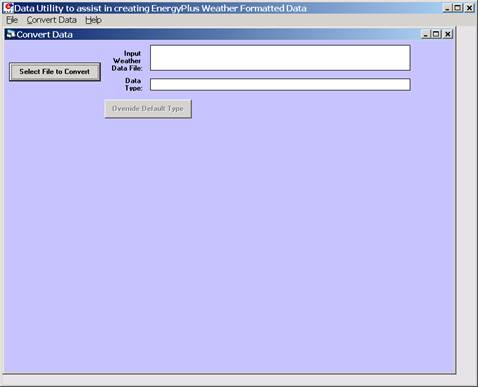
\includegraphics[width=0.9\textwidth, height=0.9\textheight, keepaspectratio=true]{media/image001.jpg}
\caption{Main menu screen of the Weather Converter Utility \protect \label{fig:main-menu-screen-of-the-weather-converter}}
\end{figure}

\subsection{File Menu}\label{file-menu-001}

The file menu has four options:

\subsubsection{Fix Out of Range Data}\label{fix-out-of-range-data}

This is a toggle option that once selected is saved in the registry with other options (for example, screen size) for the program. As shown in the IDD type description of the Weather Data, there are minimum and maximum values for several of the fields. The weather converter program can ignore these (and just report them) or it can try to fix them with appropriate values. If the option is ``checked'', then the processor will try to fix the data; if it is blank, the processor will not fix the data though it will report any out of range data that it finds.

\subsubsection{Select Delta DB Trigger}\label{select-delta-db-trigger}

Depending on the quality control and accuracy of the weather data collection, time period (usually hour to hour) changes in some data values may make the data suspect for that time period. This selection brings up the screen shown below and will allow the user some control over the actual value reporting. Note that this data is not ``fixed'', merely reported by the program in the audit output file.

\begin{figure}[hbtp] % fig 2
\centering
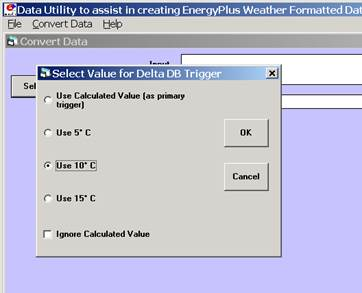
\includegraphics[width=0.9\textwidth, height=0.9\textheight, keepaspectratio=true]{media/image002.jpg}
\caption{Delta DB Trigger Selection \protect \label{fig:delta-db-trigger-selection}}
\end{figure}

Though only one ``trigger'' value is selected from this screen, consecutive values of dry-bulb temperature, dew-point temperature and wind speed are reported using appropriate calculated values. Both dew-point and wind speed use a calculated value based on mean of their values over the entire data period and standard deviation from that mean, heuristically derived.

An excerpt from the audit file is illustrative:

Average Delta DB Change = 0.78°C ; Std Dev = 0.83°C

Average Delta DP Change = 0.68°C ; Std Dev = 0.78°C

Average Delta Relative Humidity Change = 4.02\% ; Std Dev = 4.22\%

Average Delta Wind Speed Change = 0.91m/s ; Std Dev = 0.88m/s

Hourly Dry Bulb temperature change trigger = minimum of 12.13°C and 10.°C

\begin{lstlisting}
 12.13°C = calculated trigger based on mean change in dry-bulb temperature and standard deviation shown above
\end{lstlisting}

\begin{lstlisting}
 10.°C = trigger set by user
\end{lstlisting}

Here the calculated DB trigger would be 12.13°C, but the user chosen trigger is 10°C. Changes \textgreater{} = 10°C will be reported.

\begin{itemize}
\item
  Delta DB/DP Range Triggered for Apr 30
\item
  Change in DB = 11.60°C, Hour = 14
\end{itemize}

Such detail allows the user to hand edit the incoming data, if desired.

\subsubsection{Delete File}\label{delete-file}

You may use this menu option to browse your computer and delete files.

\subsubsection{Input Folder = \textgreater{} Output Folder}\label{input-folder-output-folder}

Choosing this option (a check will show and will carry over from one use to the next) sets the output folder for saving files to be the same as the input folder where the original files are located.

\subsubsection{Exit}\label{exit}

This choice exits the program.

\subsection{Converting Data}\label{converting-data}

This screen is automatically shown when you start the program - it will allow you to select raw data for processing, change the default type (based on file extension), select the kind of conversion you want, select where and what name to store for the processed data, and process the data. An ``almost'' completed screen shows:

\begin{figure}[hbtp] % fig 3
\centering
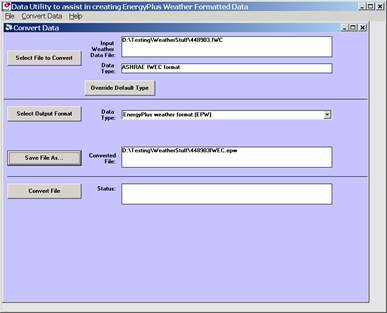
\includegraphics[width=0.9\textwidth, height=0.9\textheight, keepaspectratio=true]{media/image003.jpg}
\caption{Convert Data Screen selections \protect \label{fig:convert-data-screen-selections}}
\end{figure}

The screen is navigated by choosing the following buttons on the left portion of the screen. Interpretation from the program is shown in the status boxes on the right portion of the screen.

\subsubsection{Select File to Convert}\label{select-file-to-convert}

Selecting this command button brings up a common dialog interface that allows you to select a file for conversion from a specific set of default file extensions. These are shown in the following table. Note that you can (mostly) override the default file extension by the use of a simple DEF file and change the input file type.

% table 2
\begin{longtable}[c]{p{1.5in}p{4.5in}}
\caption{Input File Extensions with implied Data types \label{table:input-file-extensions-with-implied-data-types}} \tabularnewline
\toprule 
File Extension & Implicit Data File Type \tabularnewline
\midrule
\endfirsthead

\caption[]{Input File Extensions with implied Data types} \tabularnewline
\toprule 
File Extension & Implicit Data File Type \tabularnewline
\midrule
\endhead

LST & Processing List of Files \tabularnewline
< any >  or CST & Custom - must have "def" file as specified below \tabularnewline
EPW & EnergyPlus E/E \tabularnewline
CSV & Comma Delimited File (EPW Format) Note: special EnergyPlus CSV format. For other CSV files use the DEF file and describe the format. \tabularnewline
TM2 & TMY2 \tabularnewline
TMY & TMY \tabularnewline
IWC & IWEC \tabularnewline
WY2 & WYEC2 \tabularnewline
DAT & SAMSON \tabularnewline
FMT & DOE-2 Formatted File \tabularnewline
CLM & ESP-r Climate Formatted File \tabularnewline
ASC & BLAST ASCII \tabularnewline
SWE & SWERA \tabularnewline
WEA & Ecotect WEA file \tabularnewline
\bottomrule
\end{longtable}

Of course, the ``all files'' (*.*) may be used as well. If the file selected is not one of the above types, you will be cautioned to use the ``override default type'' button to select the correct type before proceeding. Most of the data file types are described in other publications and won't be described in detail here.

Note on the input CSV format: It is the EPW CSV format. The CSV format must mirror the output CSV format very closely. The processor expects a Location header record and the headers for the data fields as a minimum (as well as the data that supports those header fields). If you have a differently formatted file, possible comma delimited, investigate the ``custom'' format option.

The LST data type allows you to specify a list of files to be ``batch processed''. The format of this file is very simple (however, the default extensions from the preceding table \textbf{must} be used \textbf{or} you must include a ``def'' file - see below for details).

Each line of the LST file can have a columnar structure as shown in the following table or can have the input file separated from the output file with a TAB character.

% table 3
\begin{longtable}[c]{p{1.52in}p{4.47in}}
\caption{LST File Structure \label{table:lst-file-structure}} \tabularnewline
\toprule 
Columns & Contents \tabularnewline
\midrule
\endfirsthead

\caption[]{LST File Structure} \tabularnewline
\toprule 
Columns & Contents \tabularnewline
\midrule
\endhead

1-45 & Name of Input File to be Processed \tabularnewline
46-105 (or follow the first name with a \{TAB\}) & Output File with: EPW - same as output type "EPW" CSV - same as output type "CSV" Both - same as output type "both" Rpt - same as output type "rpt" \tabularnewline
106-end (or follow the second name with a \{TAB\}) & URL for KML output \tabularnewline
\bottomrule
\end{longtable}

\subsubsection{Definitions File}\label{definitions-file}

An auxiliary file, the Definitions File (extension .def) can be used to specify additional or replacement characteristics for the incoming data. This file is fully described in the section ``Definitions File \& Custom File Processing'' later in this document.

\subsubsection{Override Default Type}\label{override-default-type}

This button is used as described above to select the correct data type for a file that might have one of the standard ``default'' extensions but may, in fact, be a data file of an entirely different type. For example, the BLAST ASCII files as they exist on the BLAST CD have extensions of .dat - our default type for the SAMSON data. You must select the proper data type for your data or the processor probably won't work anywhere near what you expect.

\subsubsection{Select Output Format}\label{select-output-format}

You may select from four options of output format:

\begin{itemize}
\item
  EPW Format -- both an epw file and a statistical report file are produced
\item
  CSV Format - both a csv file and a statistical report file are produced
\item
  Both EPW and CSV - epw, csv, and statistical report files are produced
\item
  Rpt only - only a statistical report file is produced (output extension is ``stat'')
\end{itemize}

Note that the CSV file is very similar to the EPW format file but is ready to be imported into a spreadsheet program such as Excel™ and has some additional ``header'' records in front of each EPW style header record

\subsubsection{Save File As\ldots{}}\label{save-file-as}

This button allows you to select the location to save your file set from the output format selection. The utility automatically places a ``data type'' extension on the file name to show its original data file type.

Note on Save As\ldots{} Since you select the ``save as'' file name from a dialog, the processor DOES NOT warn you of overwriting previous files of the same name. In addition, if you have previously saved several types (e.g.~EPW and CSV) but this time only save the RPT - it DOES NOT create new of the others nor does it delete the previous ones.

\subsubsection{Convert File}\label{convert-file}

Pressing this button causes the processing of the data to proceed. If you choose a ``.lst'' input format, you will see messages as each once is completed and/or has errors. If you choose a single data file, you will see a similar message box once the processing is done (or has terminated due to errors).

\subsection{Help}\label{help}

No online help is available. This brings up an ``about'' box for the program.
